\begin{figure}[H]
    \centering
    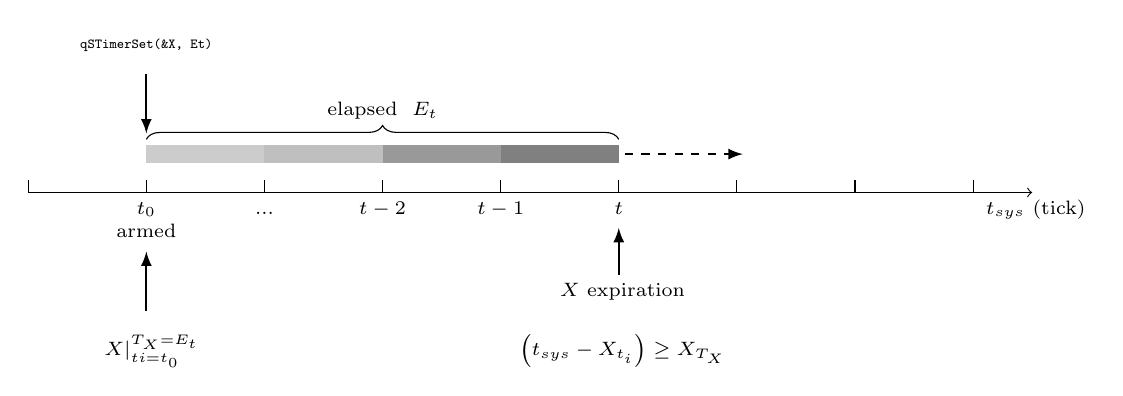
\begin{tikzpicture}[every node/.style= {font=\scriptsize, text height=1ex, text depth=.25ex,},scale=1.5]
        \draw[->] (0,0) -- (8.5,0);
        \foreach \x in {0,1,...,8}{ \draw (\x cm,3pt) -- (\x cm,0pt); }
        \node[anchor=north] at (1,0) {$t_0$};
        \node[anchor=north] at (1,-0.2) {armed};
        \node[anchor=north] at (2,0) {...};
        \node[anchor=north] at (3,0) {$t-2$};
        \node[anchor=north] at (4,0) {$t-1$};
        \node[anchor=north] at (5,0) {$t$};
        \node[anchor=north] at (6,0) {};
        \fill[gray!40] (1,0.25) rectangle (2,0.4);
        \fill[gray!50] (2,0.25) rectangle (3,0.4);
        \fill[gray!80] (3,0.25) rectangle (4,0.4);
        \fill[gray!100] (4,0.25) rectangle (5,0.4);
        \draw[black,dashed,thick,-latex] (5.05,0.325) -- (6.05,0.325);
        \draw[decorate,decoration={brace,amplitude=5pt}] (1,0.45) -- (5,0.45) node[anchor=south,midway,above=4pt] {elapsed $\ E_t$};
        \draw[black,thick,-latex] (1,1) -- (1, 0.5 ) node[anchor=north,midway,below=1pt] {};
        \draw[black,thick,-latex] (5,-0.7) -- (5, -0.3 ) node[anchor=north,midway,below=1pt] {};
        \draw[black,thick,-latex] (1,-1) -- (1, -0.5 ) node[anchor=north,midway,below=1pt] {};
        \node[anchor=north, font=\ttfamily] at (1,1.4) {\tiny qSTimerSet(\&X, Et)};
        \node[anchor=north] at (8.5,0) {$\ t_{sys}$ (tick)};
        \node[anchor=north] at (1,-1.2) {$\ \left.X\right\vert_{ti=t_0}^{T_X=E_t}$};
        \node[anchor=north] at (5,-0.7) {$\ X$ expiration};
        \node[anchor=north] at (5,-1.2) {$\ \left ( t_{sys} - X_{t_i} \right ) \geq X_{T_X}$};
    \end{tikzpicture}
    \caption{STimers operation}
    \label{fig:stimers}
\end{figure}